\chapter{BAY/DOOR} 
\label{sec:baydoor}
\lstset{style=6502Style}

The bay doors of the dropship open gradually to reveal the landing deck.
At first there is just a peek:

\begin{figure}[H]
    \centering
    \begin{adjustbox}{center}
      
\includegraphics[width=3cm]{src/baydoor_sprites/baydoor_animation_7.png}%
      \hspace{0.7cm}
      \raisebox{1.1\totalheight}{
\includegraphics[height=0.6cm]{src/baydoor_sprites/arrow.png}}
      \hspace{0.5cm}
      
\includegraphics[width=3cm]{src/baydoor_sprites/baydoor_animation_8.png}%
    \end{adjustbox}
\end{figure}
But then the teeth of the doors become visible as well and the landing deck underneath
starts to becom clear:
\begin{figure}[H]
    \centering
    \begin{adjustbox}{center}
      
\includegraphics[width=3cm]{src/baydoor_sprites/baydoor_animation_8.png}%
      \hspace{0.7cm}
      \raisebox{1.1\totalheight}{
\includegraphics[height=0.6cm]{src/baydoor_sprites/arrow.png}}
      \hspace{0.5cm}
      
\includegraphics[width=3cm]{src/baydoor_sprites/baydoor_animation_9.png}%
    \end{adjustbox}
\end{figure}

The doors begin to recede fully into their housing:

\begin{figure}[H]
    \centering
    \begin{adjustbox}{center}
      
\includegraphics[width=3cm]{src/baydoor_sprites/baydoor_animation_9.png}%
      \hspace{0.7cm}
      \raisebox{1.1\totalheight}{
\includegraphics[height=0.6cm]{src/baydoor_sprites/arrow.png}}
      \hspace{0.5cm}
      
\includegraphics[width=3cm]{src/baydoor_sprites/baydoor_animation_10.png}%
    \end{adjustbox}
\end{figure}


\clearpage
\vspace*{\fill}
\begin{figure}[H]
    \centering
    \begin{adjustbox}{width=14cm,center}
      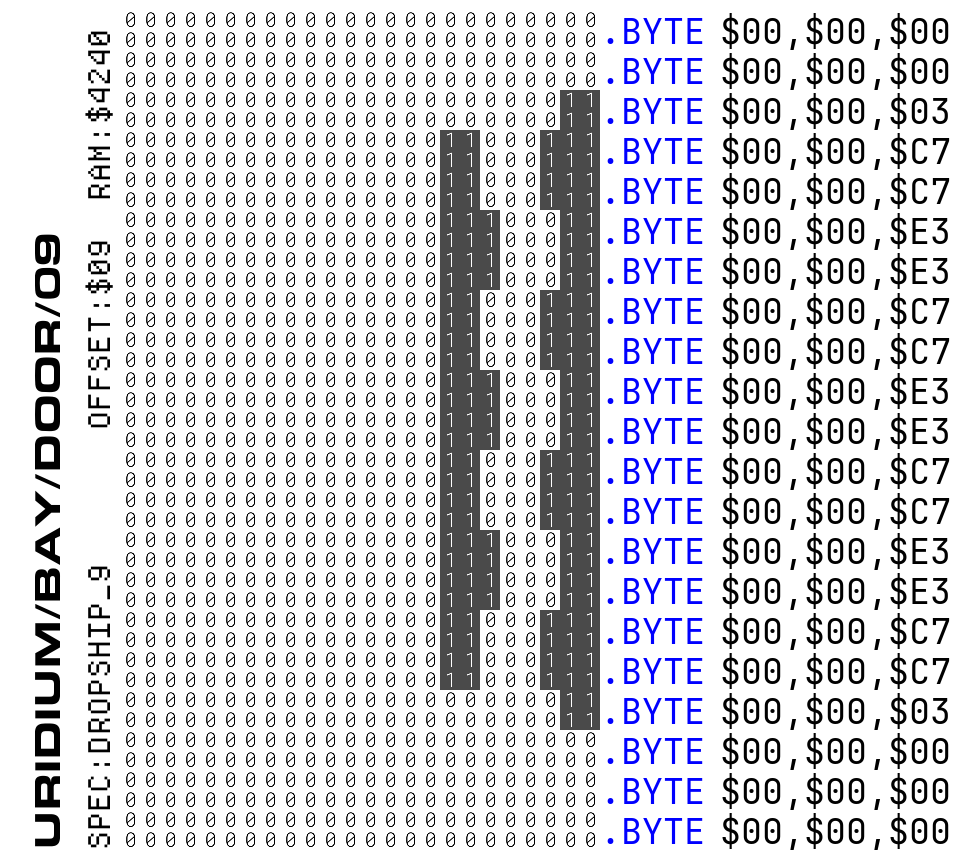
\includegraphics[width=8.8cm]{src/baydoor_diagrams/baydoor_9.png}%
      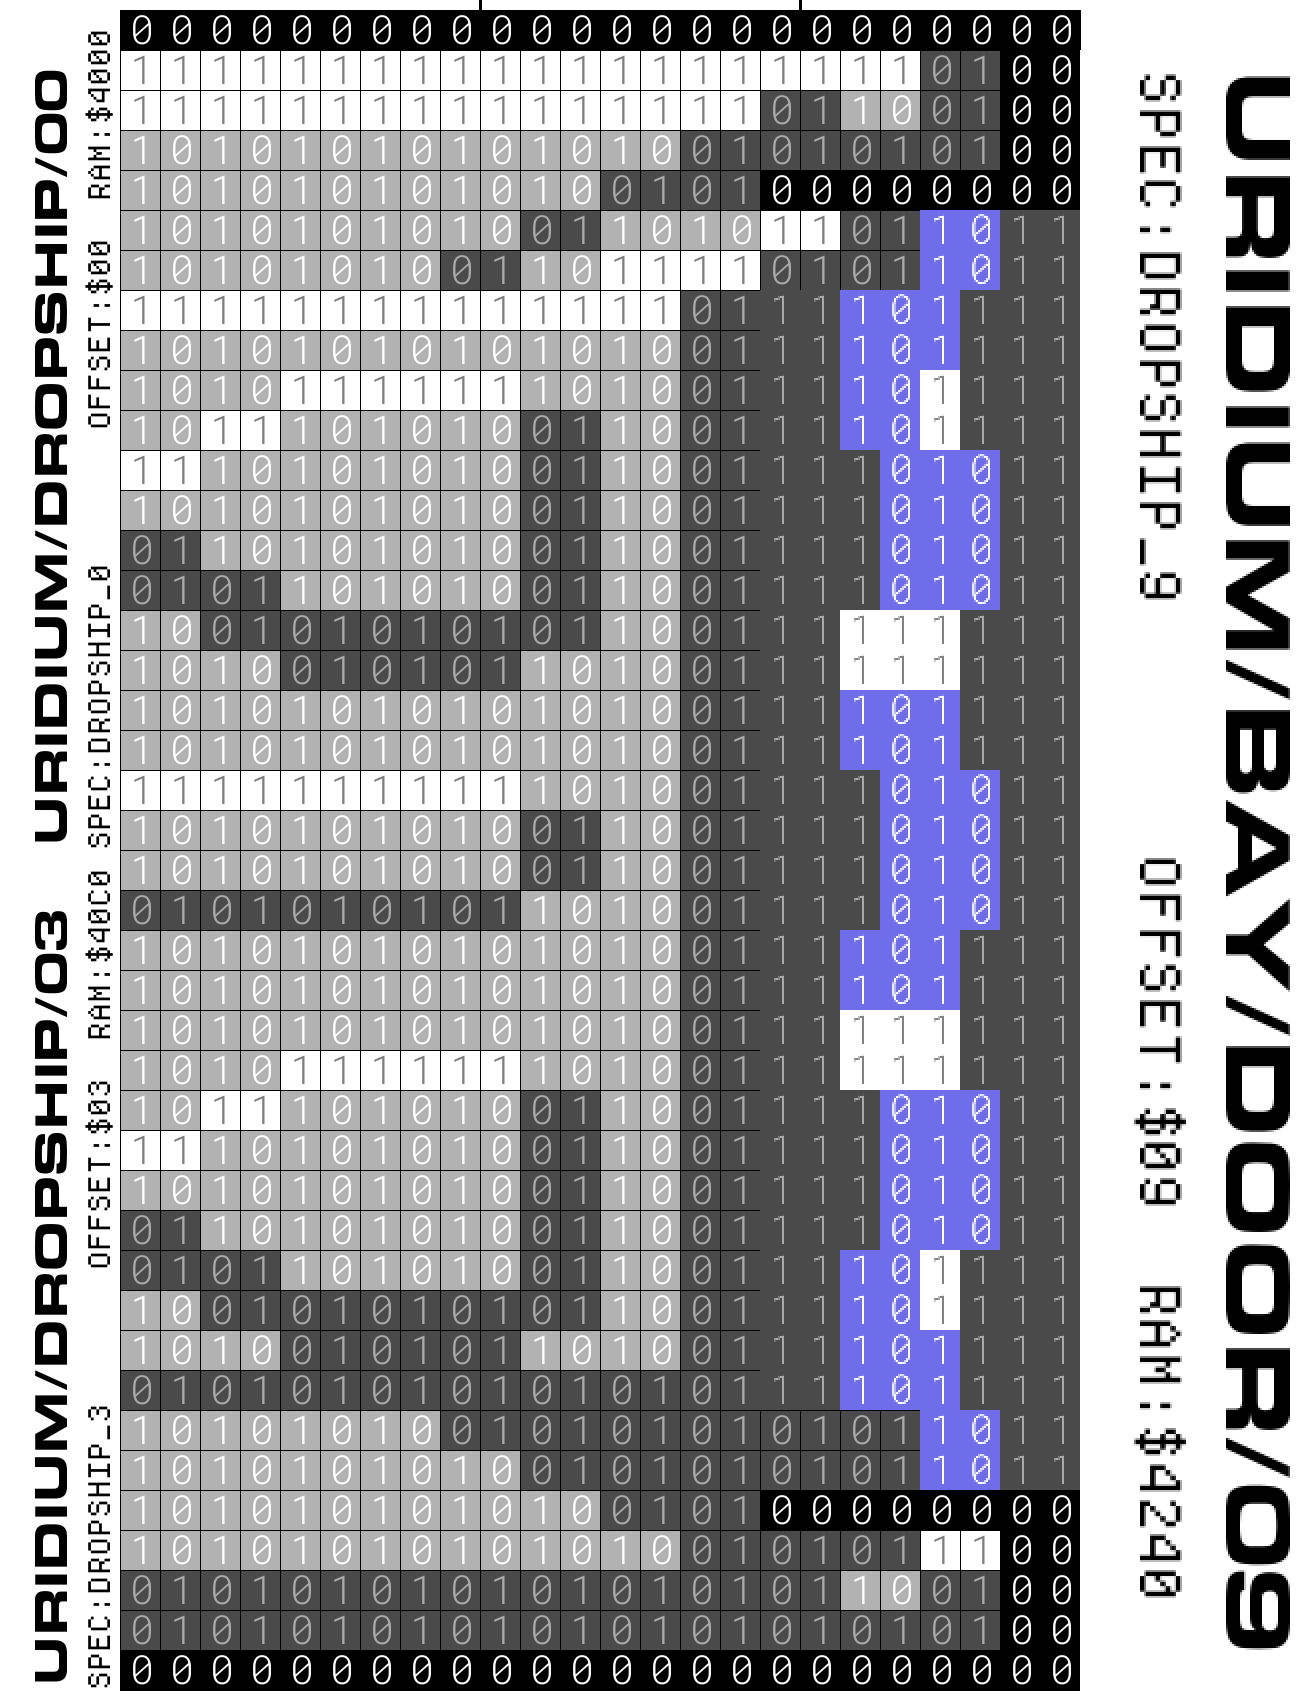
\includegraphics[width=5.8cm]{src/baydoor_diagrams/baydoor_animation_9.png}%
    \end{adjustbox}
\end{figure}
\vspace{1cm}
\begin{figure}[H]
    \centering
    \begin{adjustbox}{width=14cm,center}
      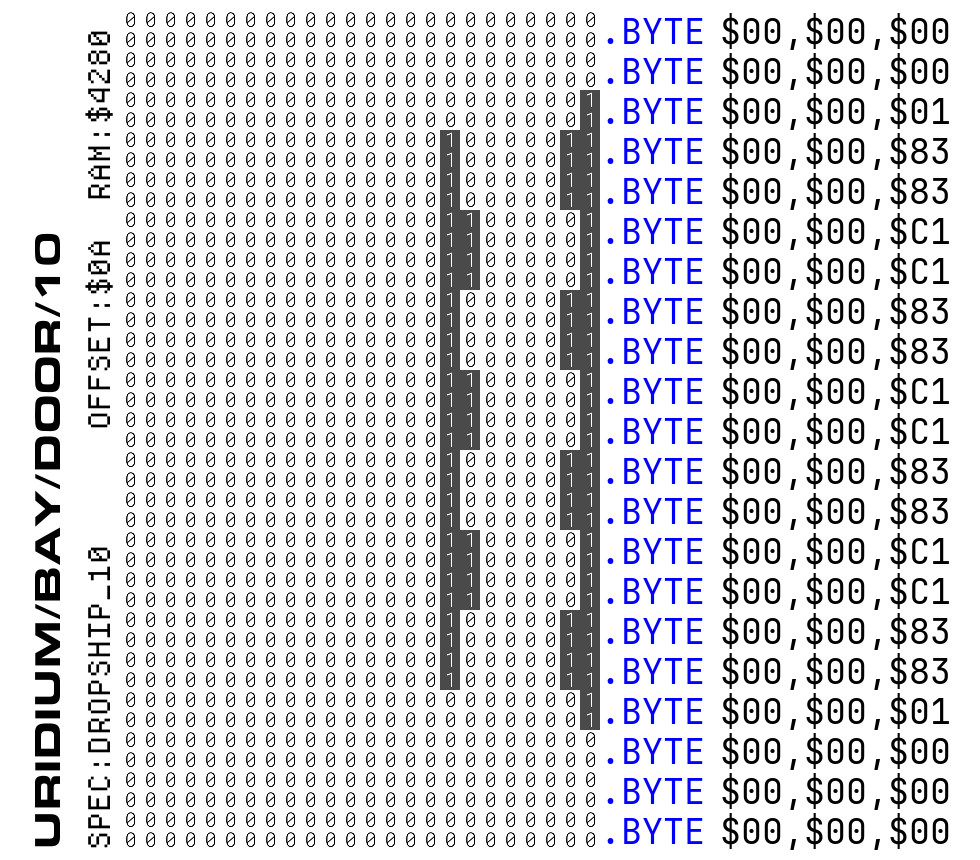
\includegraphics[width=8.8cm]{src/baydoor_diagrams/baydoor_10.png}%
      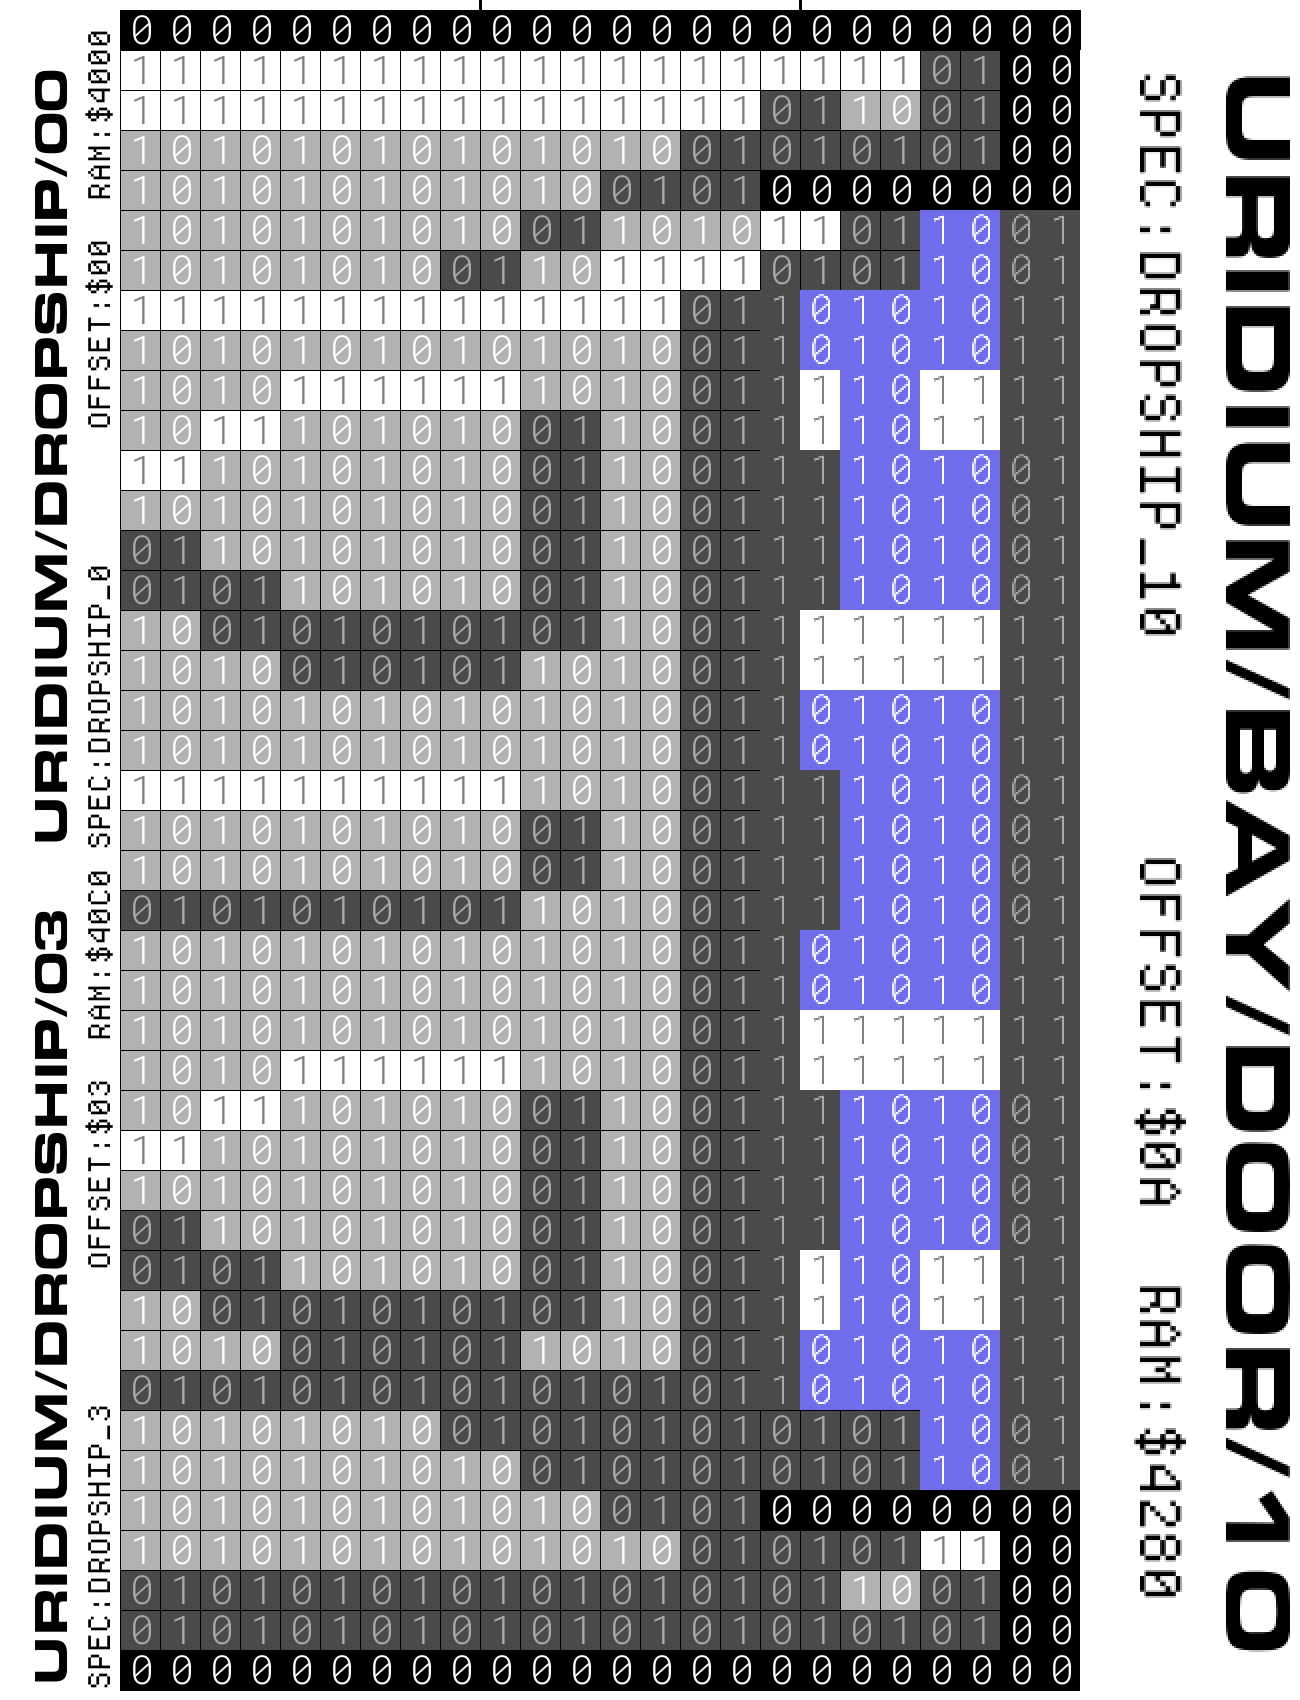
\includegraphics[width=5.8cm]{src/baydoor_diagrams/baydoor_animation_10.png}%
    \end{adjustbox}
\end{figure}
\vspace*{\fill}
\clearpage

Finally the doors recede completely and the landing deck is fully revealed:

\begin{figure}[H]
    \centering
    \begin{adjustbox}{center}
      
\includegraphics[width=3cm]{src/baydoor_sprites/baydoor_animation_10.png}%
      \hspace{0.7cm}
      \raisebox{1.1\totalheight}{
\includegraphics[height=0.6cm]{src/baydoor_sprites/arrow.png}}
      \hspace{0.5cm}
      
\includegraphics[width=3cm]{src/baydoor_sprites/baydoor_animation_11.png}%
    \end{adjustbox}
\end{figure}

In the diagrams opposite we can see that there is something subtly different about the sprites
used to achieve this effect. Close inspection of the diagrams on the left hand side shows that, unlike those used for the Manta and
the main body of the drop ship, we do not use bit-pairs to define our pixels. Instead we have
a single color, and a '\icode{1}' bit indicates a pixel while a '\icode{0}' bit indicates blank space.

This allows much greater granularity in the definition of the doors as they open - enabling the
'teeth' of the doors to be defined to a single pixel level. The diagrams on the right hand side show
how the bay door sprite is placed relative to the rest of the dropship. As we can see the bay door sprite occludes the
landing deck below, because it is drawn after it in the order we defined in \icode{loPtrsToDropShipSections} in the previous
chapter.

The switch that enables the pixel-grained rendering of the sprites is defined in the section array for the door (highlighted
with exclamation marks below). Because Multi-Color mode is turned off for the sprite every '\icode{1}'
bit in the definition is treated as a single pixel. Notice also that the X and Y position of the sprite are the
same as the \icode{landingDeckSection} we looked at earlier - because we are drawing over it in order to cover
the deck completely with the closed bay door.

\begin{lstlisting}[escapechar=\%]
bayDoorSection
  .BYTE $06      ; Sprite's index (spriteIndex).
  .BYTE $82      ; Sprite's X position.
  .BYTE $00      ; Sprite's supplemental X position.
  .BYTE $8E      ; Sprite's Y position.
  .BYTE $FF      ; Sprite Enabled.
  .BYTE $FF      ; Expand Vertical On.
  .BYTE $00      ; Display Priority vs background.
  .BYTE $00      ; !!! Multi-Color Mode OFF.
  .BYTE $00      ; Expand Horizontal Off.
  .BYTE M_GRAY3  ; Sprite color (MULTI_COLOR_1).
  .BYTE%\raisebox{-0.2\totalheight}{
\includegraphics[height=0.4cm]{src/baydoor_sprites/DROPSHIP_7.png}}%         ; Sprite Value ($07).
\end{lstlisting}

When it comes to animating the bay door opening sequence, our procedure consists of updating the sprite in place by slowly incrementing
the 'Sprite Value' that references the starting position of the closed bay door (\icode{07}  
-
\raisebox{-0.2\totalheight}{
\includegraphics[height=0.4cm]{src/baydoor_sprites/DROPSHIP_7.png}}
) 
to the final, fully open position (\icode{11} - 
\raisebox{-0.2\totalheight}{
\includegraphics[height=0.4cm]{src/baydoor_sprites/DROPSHIP_11.png}}
).
We are updating the sprite 'in place', changing nothing but the pixel content of the sprite itself. Everything
else, its position and all other parameters, stay the same.

\begin{lstlisting}
OpenBayDoorsLoop   
  LDA #$06                 ; Load the sprite index for bayDoorSection
  STA spriteIndex          ; And store it in spriteIndex.
  JSR GetCurrentSprite     ; Load the cached data for the bay door.
  INC currentSpriteValue   ; Increment the 'Sprite Value'.
  JSR DisplayCurrentSprite ; Display the new sprite.
  JSR CheckInputAndWait    ; Wait..
  JSR CheckInputAndWait    ; Keep waiting..
  JSR CheckInputAndWait    ; Keep waiting..
  LDA currentSpriteValue   ; Get the current 'Sprite Value'.
  CMP #DROPSHIP_11         ; Have we reached the last bay door sprite? 
  BCC OpenBayDoorsLoop     ; If not, keep looping.
\end{lstlisting}

The full effect of this procedure is given again below, showing us paint the closed dropship door (\icode{DROPSHIP\_7})
all the way up to the door when fully open (\icode{DROPSHIP\_11}):

\raisebox{-0.2\totalheight}{
\includegraphics[height=1.5cm]{src/baydoor_sprites/baydoor_animation_7.png}}
\hspace{0.1cm}
\raisebox{-0.2\totalheight}{
\includegraphics[height=1.5cm]{src/baydoor_sprites/baydoor_animation_8.png}}
\hspace{0.1cm}
\raisebox{-0.2\totalheight}{
\includegraphics[height=1.5cm]{src/baydoor_sprites/baydoor_animation_9.png}}
\hspace{0.1cm}
\raisebox{-0.2\totalheight}{
\includegraphics[height=1.5cm]{src/baydoor_sprites/baydoor_animation_10.png}}
\hspace{0.1cm}
\raisebox{-0.2\totalheight}{
\includegraphics[height=1.5cm]{src/baydoor_sprites/baydoor_animation_11.png}}

Once the bay doors have opened. The Manta can emerge. To achieve this we replace the sprite used for the bay door
(defined in \icode{bayDoorSection}) with a new definition we call \icode{mantaTakingOff}. Notice that the 'index'
of \icode{'06'} is the same in this definition but we change sprite we're referencing with the Manta's sprite, as well as enabling
multi-color mode to ensure we draw the Manta correctly. 'Replacing' the bay door in this way ensure that it occurs
in the same position as the doors in relation to the other objects, i.e. above the landing deck but below the rest of the 
craft. This is essential to achieve the 'emerging' effect:

\begin{lstlisting}[escapechar=\%]
mantaTakingOff
  .BYTE $06      ; Sprite's index (spriteIndex).
  .BYTE $70      ; Sprite's X position.
  .BYTE $00      ; Sprite's supplemental X position.
  .BYTE $98      ; Sprite's Y position.
  .BYTE $FF      ; Sprite Enabled.
  .BYTE $00      ; Expand Vertical Off.
  .BYTE $00      ; Display Priority vs background.
  .BYTE $FF      ; Multi-Color Mode On.
  .BYTE $00      ; Expand Horizontal Off.
  .BYTE M_BLACK  ; Sprite color (MULTI_COLOR_1).
  .BYTE %\raisebox{-0.2\totalheight}{
\includegraphics[height=0.4cm]{src/baydoor_sprites/manta_animation_sprite.png}}%      ; Sprite Value ($59).
\end{lstlisting}

To swap out \icode{bayDoorSection} with \icode{mantaTakingOff} we must load \icode{mantaTakingOff} into memory. The fact that
it has the same index of \icode{'06'} ensures that we replace \icode{bayDoorSection}:
\begin{lstlisting}
  ; Replace the bay door sprite with the manta sprite.
  JSR CheckInputAndWait
  LDA hiPtrToMantaTakingOff
  STA spriteVariablesHiPtr
  LDA loPtrToMantaTakingOff
  STA spriteVariablesLoPtr
  JSR LoadSpriteVariablesAndDisplay
\end{lstlisting}

With this done we can now perform the animation. This consists of loading the sprite, updating its X position, and
redisplaying it. We then repeat this process until the Manta reaches the middle of the screen, which is around pixel
position 170:

\begin{lstlisting}
MoveMantaOutOfDropShip   
  LDA #$06                 ; Load the sprite index for mantaTakingOff
  STA spriteIndex          ; And store it in spriteIndex.
  JSR GetCurrentSprite     ; Load the cached data for the manta.
  INC currentSpriteXPos    ; Increment the Manta's X position.
  JSR DisplayCurrentSprite ; Display the manta in the new position.
  JSR CheckInputAndWait    ; Wait..
  JSR CheckInputAndWait    ; Keep waiting.. 
  LDA currentSpriteXPos    ; Get the Manta's current position.
  CMP #170                 ; Loop until it reaches 170.
  BCC MoveMantaOutOfDropShip
\end{lstlisting}

The effect is illustrated below. An interesting detail, which you may have noticed, is that the Manta is the
wrong colour. Notice that it's detailing is grey rather than yellow. 

\raisebox{-0.2\totalheight}{
\includegraphics[height=1.5cm]{src/baydoor_sprites/manta_animation_0.png}}
\hspace{0.1cm}
\raisebox{-0.2\totalheight}{
\includegraphics[height=1.5cm]{src/baydoor_sprites/manta_animation_5.png}}
\hspace{0.1cm}
\raisebox{-0.2\totalheight}{
\includegraphics[height=1.5cm]{src/baydoor_sprites/manta_animation_10.png}}
\hspace{0.1cm}
\raisebox{-0.2\totalheight}{
\includegraphics[height=1.5cm]{src/baydoor_sprites/manta_animation_15.png}}
\hspace{0.1cm}
\raisebox{-0.2\totalheight}{
\includegraphics[height=1.5cm]{src/baydoor_sprites/manta_animation_20.png}}
\hspace{0.1cm}
\raisebox{-0.2\totalheight}{
\includegraphics[height=1.5cm]{src/baydoor_sprites/manta_animation_25.png}}

This isn't entirely deliberate - the 
color immediately changes back to yellow once the game starts - so it would have to be an either oversight or the result
of an unavoidable constraint. It happens to be the latter - the color of the detailing is determined by
a color value shared by all sprites. This isn't a problem during gameplay as the enemies also use this yellow
color value. However during the dropship sequence this shared color is a dull grey, the shadow tones used to
give depth to the dropship. As a result, during deployment the Manta must carry gray rather than yellow racing stripes.
Once the player takes control, however, it can revert immediately to the color it shares with the enemies. On the first 
level, this is yellow, but this color also changes in the later stages of the game to pink, blue, and so on.

